\subsection{MDPs for Intensity Maximization}\label{sec:mdp}
In~\cite{capuano2023temporl}, the authors formulate pulse shaping as a control problem in a Markov Decision Process (MDP), \( \mathcal{M} \). In this work, we extend their formulation to the case where the environment dynamics are influenced by an unobserved latent variable, leading to a \textit{Latent MDP} (LMDP)~\citep{chen2021understanding}, denoted as \(\mathcal{M}_\xi = \{\mathcal{S}, \mathcal{A}, \mathbb{P}_\xi, r, \rho, \gamma\}\). Here, \( \xi \) is a realization of a latent random vector \( \Xi \), such that \(\xi \sim \Xi : \supp(\Xi) \subseteq \mathbb{R}^{|\xi|}\), parametrizing the transition dynamics \( \mathbb{P}_\xi \). Crucially, the agent does not directly observe \( \xi \) at test time (i.e.~the real world).
Conversely, we assume that parameters \( \xi \) may be accessed when training in simulation.
We argue the LMDP framework is particularly well-suited for pulse shaping in a non-stationary setting due to the presence of hidden variations in the system's dynamics. In practical scenarios, an agent must adapt to an unknown experimental condition which can be modeled as \( \xi \), while iteratively refining its control \( \psi \). As \( \psi \) is physically translated into temperature gradients applied to an optical fiber, the choice of \( \psi_t \) must account for past applied controls, particularly \( \psi_{t-1} \), to prevent excessive one-step temperature variations, which may endanger the fiber. Moreover, the day-to-day fluctuations in HPL systems can be captured through \( \Xi\), modeling the inherent non-stationarity of experimental conditions. Further, by incorporating a distribution over the starting condition of the system, \( \psi_0 \sim \rho \), the pulse shaping problem's sequential nature becomes evident---starting from a randomly sampled experimental condition, the agent must iteratively apply controls \(\psi\) while dealing with incomplete knowledge of the system dynamics.
% The additional randomness introduced through \( \xi \) further enhances the stochasticity of the environment, increasing the need for robust and adaptive policies. Finally, the problem of policy transferability across different latent environments remains an active research area in RL and meta-learning, and by adopting the LMDP framework, we directly position our work to benefit from advancements in this domain.
Inspired by the domain randomization and meta-learning literatures, we therefore aim at learning control policies that are robust and adaptive to unknown, hidden contexts.

\paragraph{State space ($\mathcal S$)}
Ideally, one could access the temporal profile of the pulse to describe the status of the laser system. Indeed, the temporal profile $\chi(\psi)$ contains all the information needed to maximize peak intensity, including pulse energy and duration.
However, obtaining high-fidelity temporal profiles of ultra-short laser pulses in practice is a challenging task~\citep{trebino1993using, trebino1997measuring}.
%~\cite{zahavy2018deep} propose adopting CNNs to reconstruct $\chi$ starting directly from experimentally-available FROG traces, collected as diagnostic tools in most laser systems.
Here, we instead leverage FROG traces as proxy for state information.
As FROG traces contain enough information to reconstruct temporal profiles~\citep{zahavy2018deep}, we argue they could also be used as direct inputs to a control policy aiming at maximizing peak intensity. Further, using FROG traces would be practically convenient given the availability of FROG detection devices in most HPL systems, and prevent the need for an intermediate step in the pulse shaping feedback loop to reconstruct \( \chi \) from its associated FROG trace, \( \Phi \). Hence, we directly include FROG traces $\Phi_t$ in our state space. We complement states $s_t$ with the vector of dispersion coefficients $\psi_t$ and the action taken in the previous timestep, $a_{t-1}$, giving $s_t = \{ \Phi_t, \psi_t, a_{t-1} \}$, as they all are information available at test time.
% dim of FROG?

\paragraph{Action space ($\mathcal A$)}
As we are concerned with real world applicability of our method, we design an action space that is inherently machine-safe, and that can prevent erratically changing the control applied at test time. In this, we consider varying dispersion coefficients within predetermined boundaries defined at the level of the grated optical fiber, i.e. \( \psi_t \in [\psi_{\text{min}}, \psi_\text{max}]: c = \vert\psi_{\text{min}} - \psi_\text{max} \vert \). Actions are then defined as $a_t \in [-\alpha c, +\alpha c]$, with $\alpha$ being an arbitrary fraction of the total nominal range \( c \). In our method, we set $\alpha=0.1$, thus never changing $\psi$ in one step by more than 10\% of the total possible variation.

\paragraph{Environment dynamics ($\mathbb P_\xi: \mathcal S \times \mathcal A \times S \mapsto \mathbb{R}^+)$}
Inspired by the successes of in-simulation learning in robotics~\citep{antonova2017reinforcement, akkaya2019solving, tiboni2023domain}, we employ simulations of the pump chain process while training a policy to control it. This allows us to scale the number of samples available at training time to amounts that are simply unfeasible on real-world laser hardware.
We refer the reader to~\cite{paschotta2008field} for an in-detail coverage of the phase accumulation process, useful to describing the model for state-action-next transitions, $\mathbb P_\xi (s_{t+1}\vert s_t, a_t)$. Here, we wish to pose particular emphasis on the role of $\xi$ on $\mathbb P_\xi$. Figure~\ref{fig:b_integral} shows how different $\xi_i$ can lead to significantly different pulses when applying the same $\psi$. In particular,~\ref{fig:b_integral} simulates the impact of randomizing the parameter regulating non-linear phase accumulation during amplification. This parameter is typically referred to as \emph{B-integral}, and indicated with $B$. 
In HPL systems, one cannot typically assume to have control over $B$ but indirectly: non-linear effects become more evident when higher-intensity pulses are propagated through non-linear crystal, which induces non-stationarity in $B$. Further, precisely estimating $B$ at a given time is a challenging tasks, prone to imprecision and which can have drastic impacts on the peak intensity achieved (Figure~\ref{fig:dynamics_peak_intensity}).

% \begin{figure}
%     \centering
%     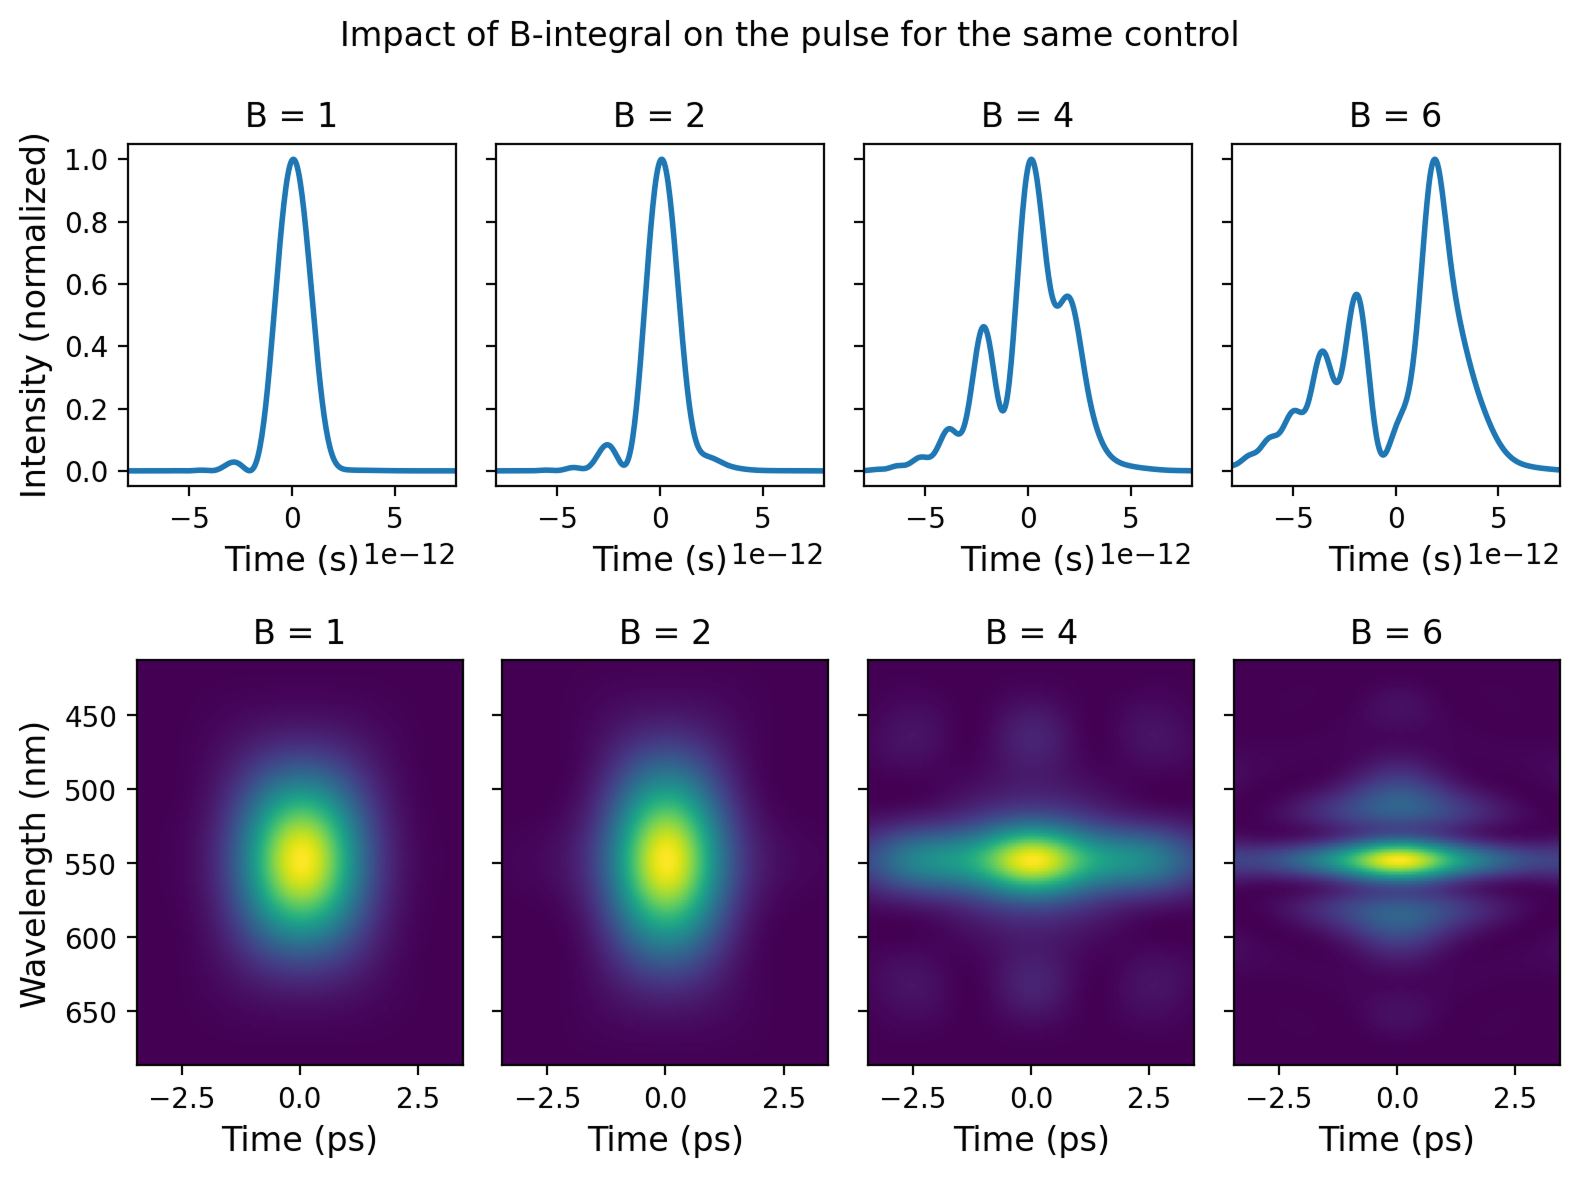
\includegraphics[width=0.8\linewidth]{images/B_integral.png}
%     \caption{Impact of the B-integral parameter on the temporal profile (top) and FROG trace (bottom) for the same control, \( \psi \). As it regulates non-linear phase accumulation, increasing B-integral modulates the pulse in time, resulting in longer pulses and thus dispersing intensity.}
%     \label{fig:b_integral}
    
% \end{figure}
\begin{figure}
    \centering
    \begin{minipage}{0.58\linewidth}
        \centering
        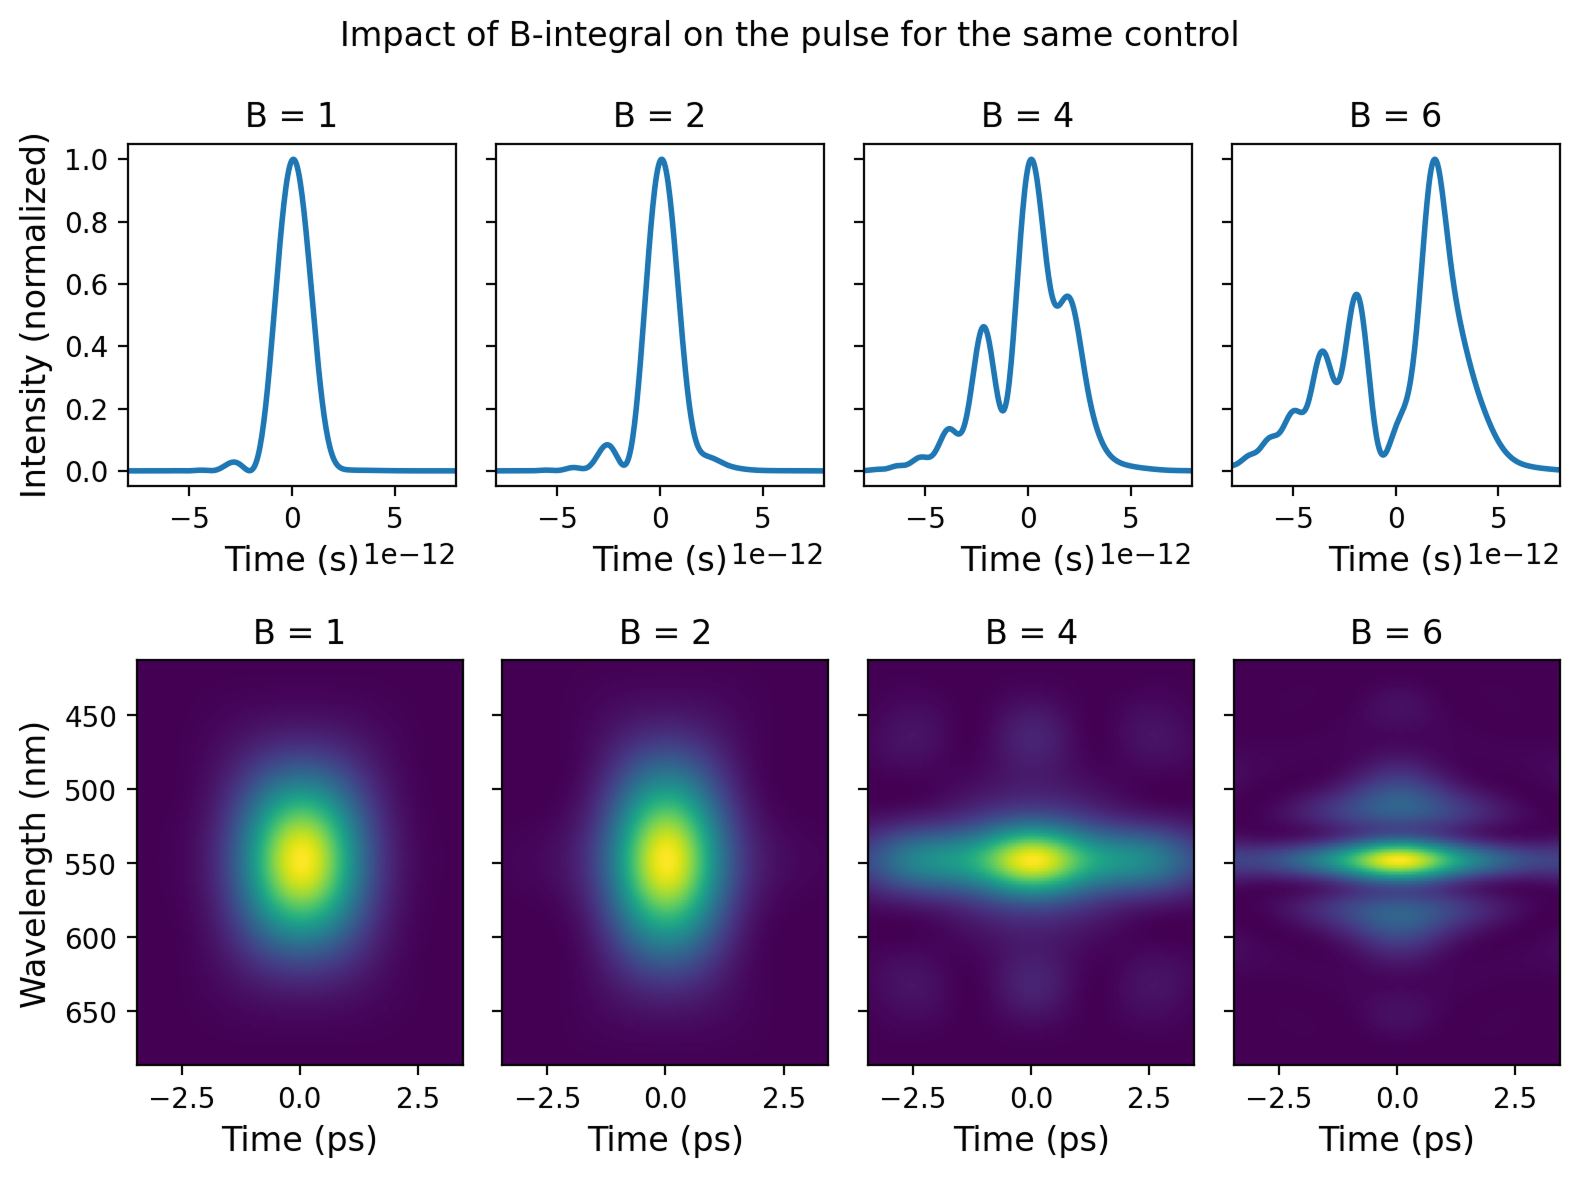
\includegraphics[width=\linewidth]{images/B_integral.png}
        \caption{Impact of the B-integral parameter on the temporal profile (top) and FROG trace (bottom).}
        \label{fig:b_integral}
    \end{minipage}
    \hfill
    \begin{minipage}{0.4\linewidth}
        \centering
        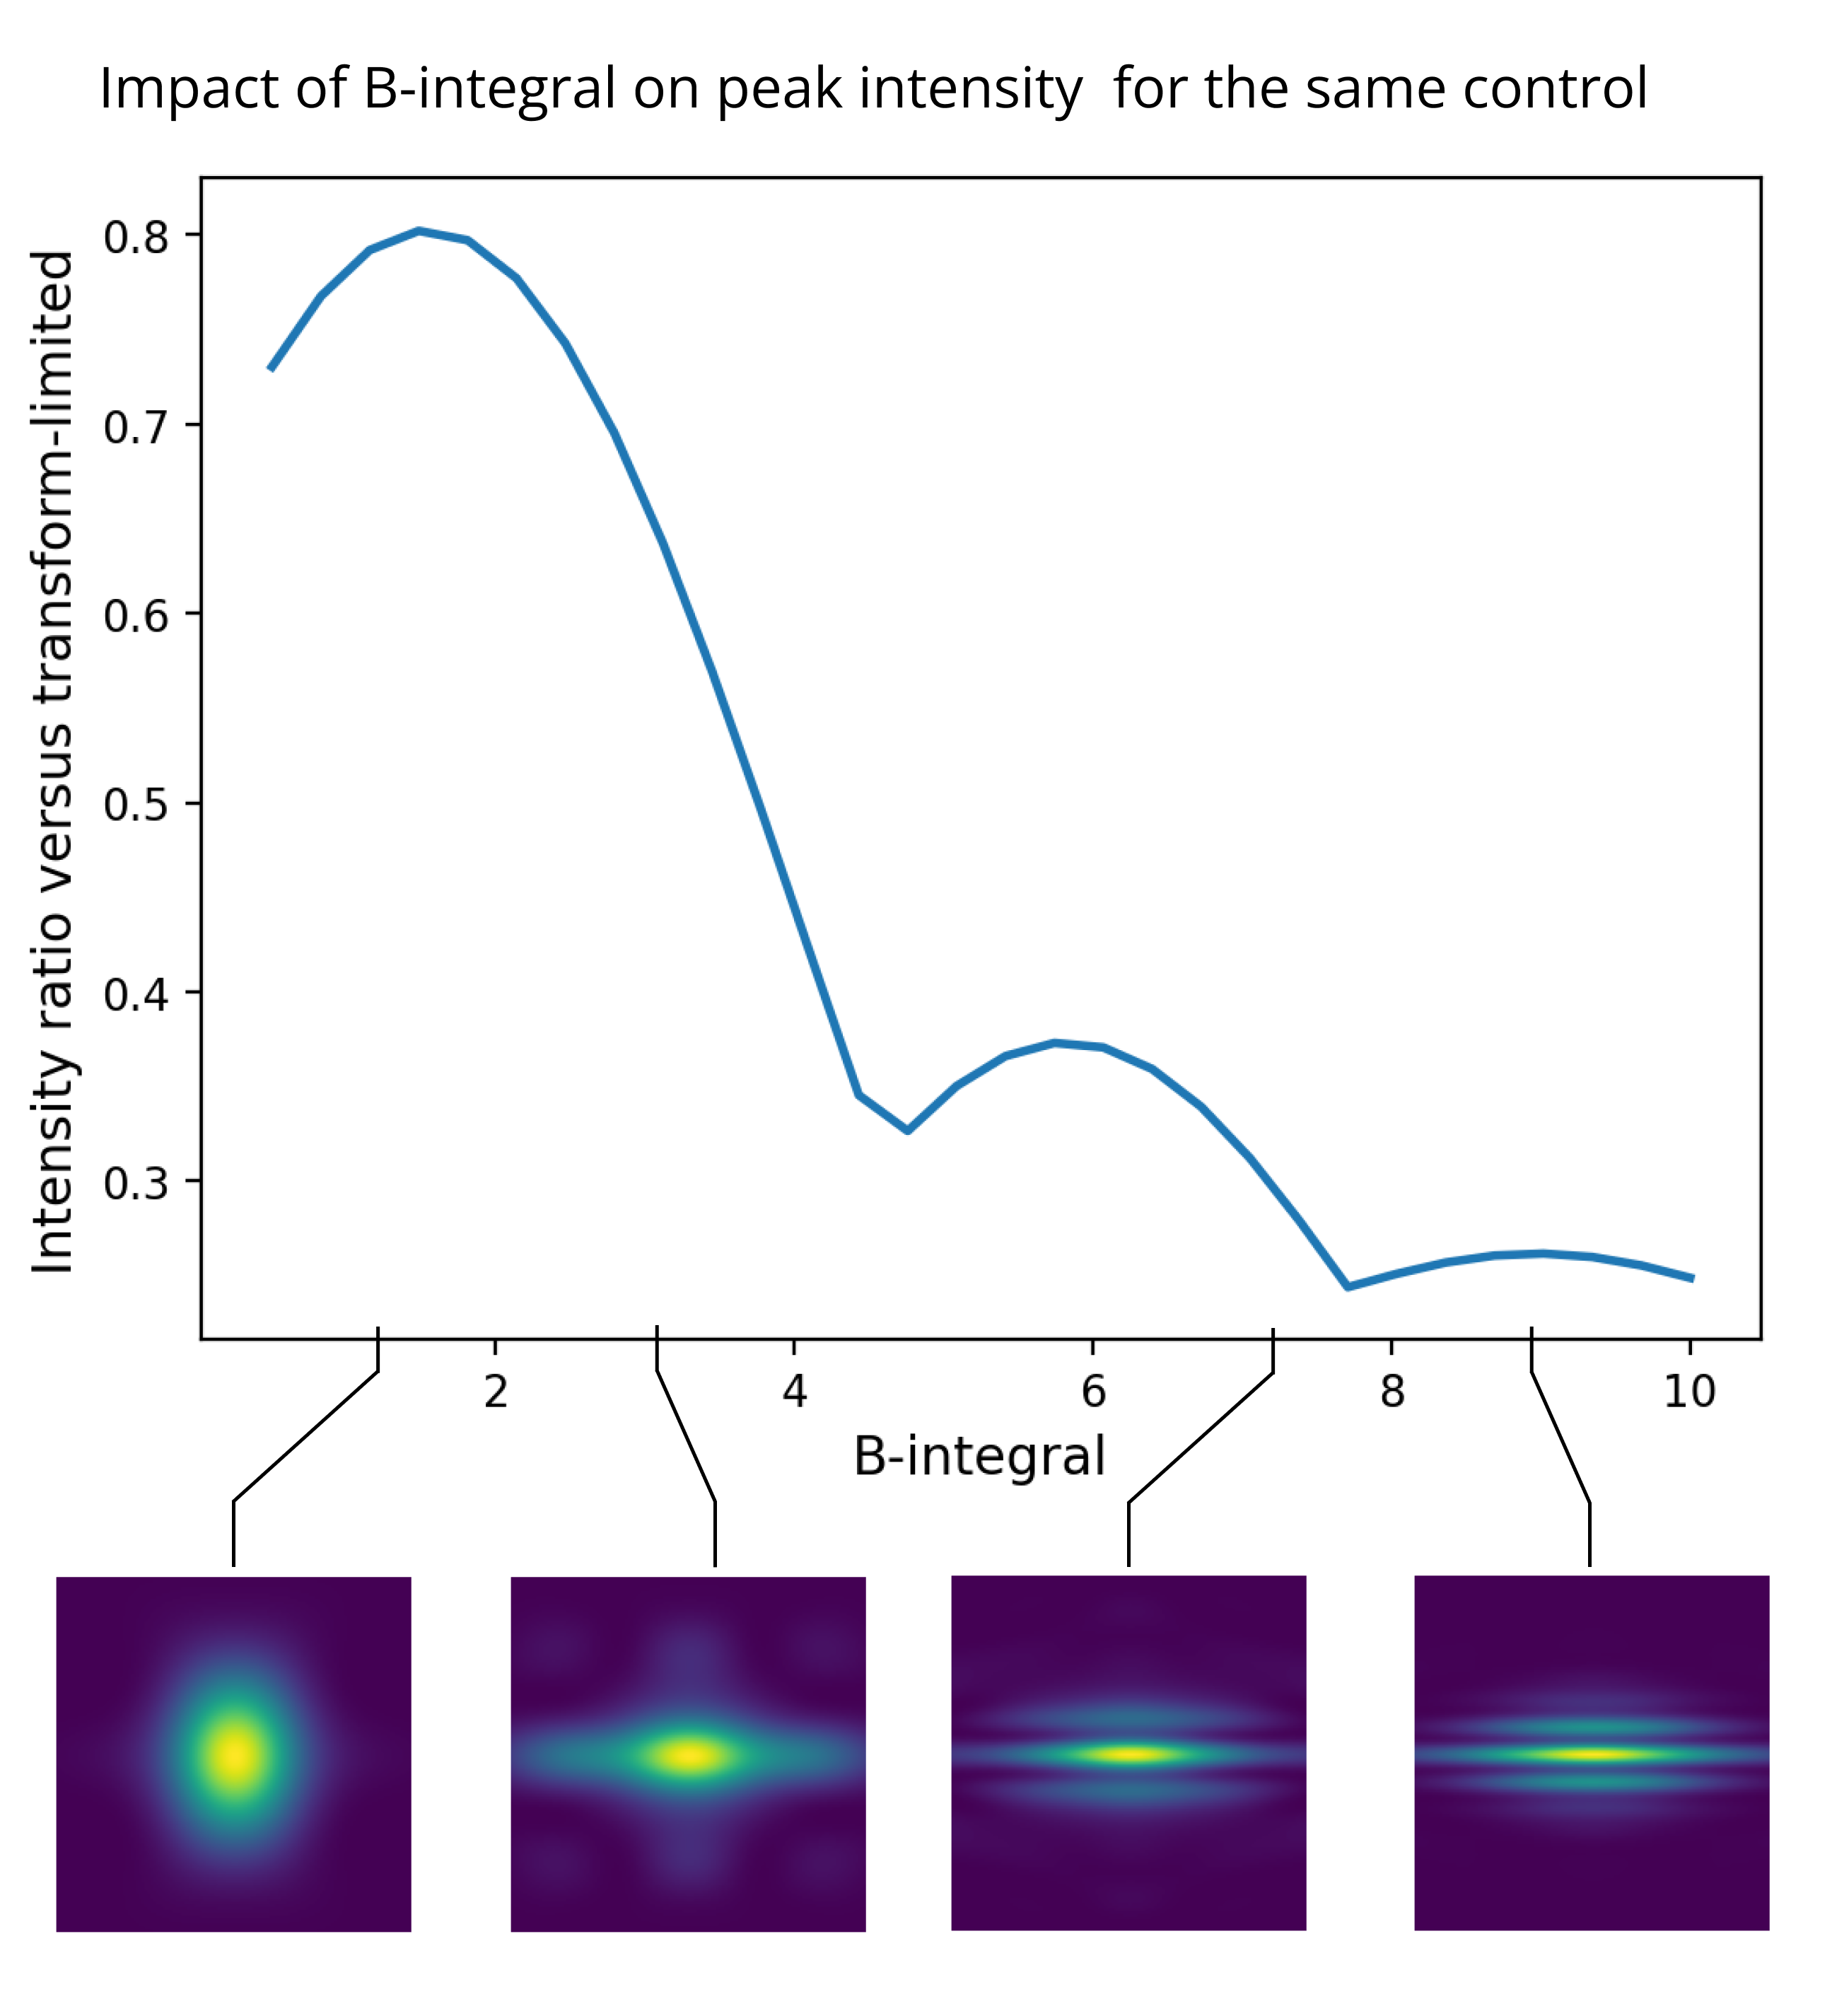
\includegraphics[width=\linewidth]{images/peak_intensity.png}
        \caption{Impact of longer pulses on the peak intensity conveyed, measured as a fraction of $I_{TL}$.}
        \label{fig:dynamics_peak_intensity}
    \end{minipage}
\end{figure}

\paragraph{Reward function $r$, Starting condition $\rho$ and discount factor $\gamma$}
We exploit our knowledge of HPL systems to design a reward function defined as the ratio between the current-pulse peak intensity $I_t^*$ and the highest intensity possibly obtainable, $I_{TL}$ achieved by so-called \emph{Transform-Limited} pulses, yielding \(r_t(s_t, a_t, s_{t+1}) = \frac{I_t}{I_{TL}} \in [0,1] \ \forall t \). In the absence of non-linear effects due to amplification, one would impose a phase on the stretcher that is opposite to the compressor's, $\varphi_s(\omega) = - \varphi_c(\omega)$ so as to maximize intensity. As non-linearity is induced, it is reasonable to look for solutions in a neighborhood of the compressor's dispersion coefficients. Thus, one can use a multivariate normal distribution $\mathcal N(-\psi_c, \epsilon \mathbb I)$ with mean $-\psi_c$ and diagonal variance-covariance matrix. Lastly, we employed an episodic framework for this problem, fixing the number of total interactions to $T=20$, and used a discount factor of $\gamma=0.9$.

\subsection{Soft Actor Critic (SAC)}
Because we run training in simulation, we are able to drastically scale the experience available to the agent. With that being said, our simulation routine requires non-trivial computation, such as obtaining \( \Phi_t \) from \( \psi_t \). Thus, we limit ourselves to the generally more sample-efficient end of DRL, and refrain from using purely on-policy methods, such as~\cite{schulman2015trust, schulman2017proximal}.
% As we work towards practical applicability, we value the possibility of deriving deterministic control policies, which in turn makes algorithms such as DDPG~\citep{lillicrap2015continuous} and SAC~\citep{haarnoja2018soft} particularly appealing to us.
% As we target LMDPs with varying dynamics, we are particularly interested in learning policies exploring robustly, and thus identify SAC as our algorithm of choice.

SAC is an off-policy DRL algorithm
%designed for continuous action spaces
that leverages the power of deep function approximators to learn Q-functions (policy evaluation) that generalize across high-dimensional state-action spaces. Then, a stochastic policy is iteratively learned by explicitly maximizing the current Q-function estimate (policy improvement). 
%where the policy is obtained deterministically starting from the Q-function developed by the agent.
Interestingly, the Q-function itself is learned in a maximum entropy framework, leading to improved exploration and overall more effective learning over competing methods such as DDPG~\citep{haarnoja2018soft}. In this work, we implement both \emph{vanilla-SAC} and \emph{asymmetric-SAC}. The latter makes use of additional privileged information about the dynamics \( \xi \) while training. Notably, this information is yet not accessible by the policy, which is only conditioned on the current state.
% In the setting of domain transferability it is typical to provide approximators of the Q-functions---not queried at test time---with privileged information about the dynamics $\xi$.
The adoption of this asymmetric paradigm has proven empirically effective in easing the training process, by providing full information to the critic networks which are nevertheless not queried at test time~\citep{akkaya2019solving}.

\subsection{Domain Randomization (DR)}
To improve on the generalization of the control policy over unknown test conditions $\xi \sim \Xi^{real} $, we train a control policy in simulation by sampling dynamics parameters from an arbitrary auxiliary distribution $\Xi$. Particularly, we compare two popular methods for choosing said distribution over $\xi$, namely Uniform Domain Randomization (UDR)~\citep{tobin2017domain, sadeghi2016cad2rl} and Domain Randomization via Entropy Maximization (DORAEMON)~\citep{tiboni2023domain}.

UDR models \( \Xi \) as a uniform distribution over manually defined bounds \( [\xi_{\min}, \xi_{\max}] \).
% While training, environments parametrized by $\xi \sim \mathcal U(\xi_{\min}, \xi_{\max})$ are sampled.
Crucially, identifying the bounds to use in training is an inherently brittle process: too-narrow bounds could hinder generalization, by not providing sufficient diversity over training. On the other hand, too-wide bounds can yield over-regularization, and thus result in reduced performance at test time. In the context of our application, experimentalists at ease with the specific pump-chain laser considered in this work estimate \( B \approx B_{\text{est}} = 2 \). Thus, we train a UDR policy in simulation by using $\xi = B \sim \mathcal U(1.5, 2.5)$, which is roughly equivalent to allowing misspecification of up to 25\% error.
% While it can be justified considering the low probability that human experts misestimate the value of B-integral by more than 25\%, the choice of the B-integral coefficient to use in simulation still requires tuning due the reality gap~\citep{tobin2017domain}.
However, even assuming access to ground-truth bounds, the probability mass of \( B \) is unlikely to be uniformly distributed on large supports---this would severely impact the performance of the system on a day to day basis. Conversely, it is reasonable to expect mass to be concentrated around some value within a possibly larger support, further away from \( B_{\text{est}} \).
% In principle, we could train an agent on an environment parametrized by a new distribution $\Xi: \supp (\Xi) = [1, 3.5]$ by using Beta distributions, and adjusting them over training shifting mass to be more or less concentrated.
In DORAEMON~\cite{tiboni2023domain}, the authors resolve the ambiguities in defining the training distribution by employing the principle of maximum entropy~\citep{jaynes1957information}. In other words, one could simply define a success indicator for the task, and seek for the maximum entropy training distribution \( \Xi \) that satisfies a lower bound on the success rate.
%
More precisely, DORAEMON solves this problem with a curriculum of evolving Beta distributions \( \Xi_k \sim \Beta(a_k, b_k) \).
%, conditioning the sequence \(\{\Xi_k\}_{k=1}^K\) to vary based on the agent's performance on \( \Xi_k \).
In line with~\cite{tiboni2023domain}, we apply DORAEMON as an implicit meta-learning strategy for training adaptive policies over hidden dynamics parameters. We define a custom success indicator function on trajectories \( \tau_{\xi_k} \): terminal-state pulses \( \chi(\psi_T) \) must convey at least 65\% of the TL-intensity for the respective episode to be considered successful.
%In DORAEMON, when more than a fraction---50\% in our experiments---of the test episodes are declared successful, $\Xi_k$ is updated in the direction of entropy maximization.
As a result, our implementation yields an automatic curriculum over DR distributions \( \Xi \) at training time such that entropy grows so long as the success rate is above \( 50 \)\%---as in the original paper.  
%that is automatically updated conditioned on the performance achieved under the current dynamics.
%one dynamics.